%Conclusion
%\subsection{Financial Industry Leverage: Past Decades}
% Investors Buying on Leverage from the financial firm, amount of funds that have to be held as margin for a leveraged purchase of securities!!!

%
%Could the leveraging approach to drop in profits have been averted.....??Did the inversion and leverage lead to the drop in profitability....?     

%Financial Industry Leverage: Past Decades

%The relation between short-horizon investor risk aversion and asset pricing is more complicated\cite{Gallmeyer}

There were long-term forces at play leading up to the financial crisis of 2008.  The trends seen in margin accounts subfigure \ref{fig:debitMargin}, is indicative of the rise in investor leverage and the effects of repealing Glass-Steagall.  The acceleration of debit balances from 1995 on has driven the divergence of M2 and M1 money supply indicators, and has contributed to the rise of one other major indicator.  The bubble in subfigure \ref{fig:bubble} spans several decades and burst all of a sudden in the financial crisis of 2008.  The bubble in subfigure \ref{fig:bubble} shows the ratio of Financial Company Owned \& Managed Receivables to Total Commercial Bank Liabilities.  The bubble is indicative of distorted valuation in financial firm assets.  This increases the systemic risk of a massive fire sale of misplaced assets.  

\begin{figure}[H]
\centering
\begin{subfigure}{.5\textwidth}
  \centering
  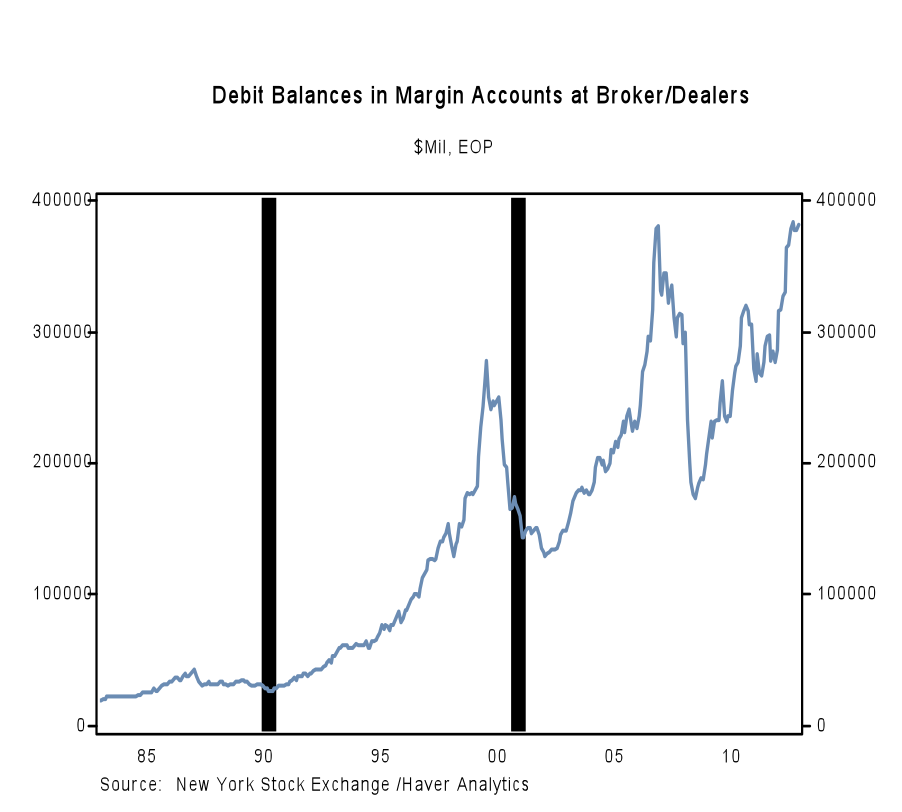
\includegraphics[width=0.9\linewidth]{figure/DebitBalancesMargin.png}
  \caption{Buying on Margin: On Behalf of Clients}
  \label{fig:debitMargin}
\end{subfigure}%
\begin{subfigure}{.5\textwidth}
  \centering
  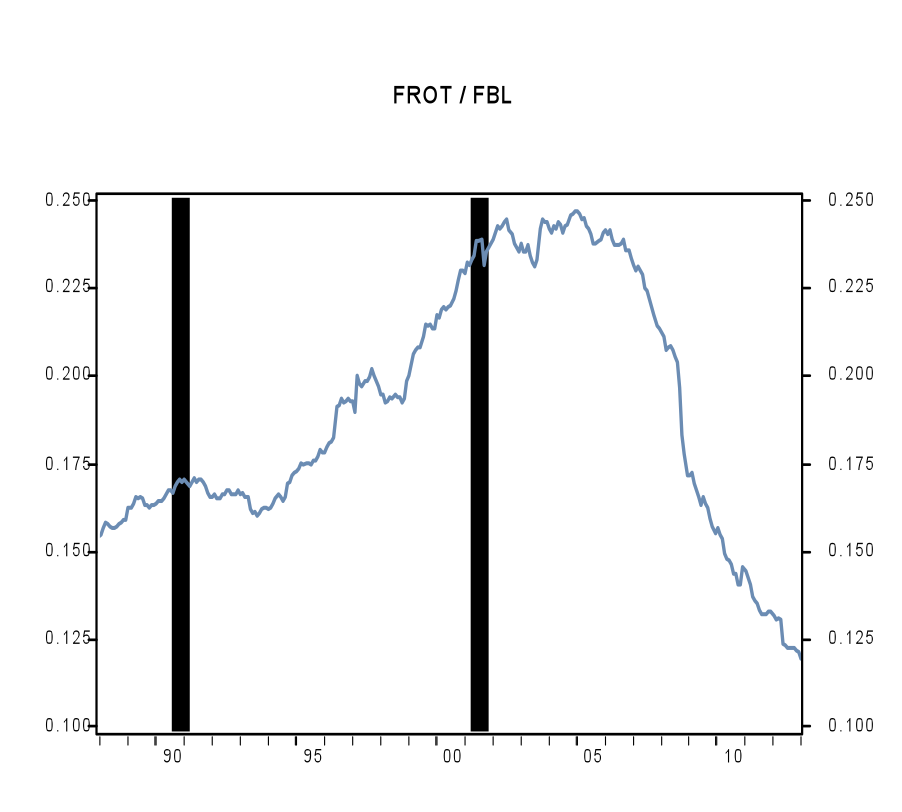
\includegraphics[width=1.0\linewidth]{figure/Bubble.png}
  \caption{Asset Value Bubble}
  \label{fig:bubble}
\end{subfigure}
\caption{Striving for Profitability}
\label{fig:NEW2}
\end{figure}
%Hedging bubble, Total Commercial Banking Liabilities Financial company owned and managed
%Hedging bubble, incorrect valuations







%%%%%%%%%%%%%%%%%%%%%%%%
%%%%%%%%%%%%%%%%%%%%%%%%

The divergence of M2 from M1 is larger than business cycle recessions, and pertains explicitly to the rise and fall of TBTF as it pertains to financial firms.  The financial market for short-term funding will peak in quantity and the rate requested by a lender will spike prior to an economic downturn.  The combination of these events precedes unprecedented government intervention, aimed at liquidating financial firm long-term and mis-priced asset positions.  The combination of these events is going to continue on an upward long-wave trend as is illustrated by the left most graph in figure \ref{fig:TBTF} below.

\begin{figure}[H]
\centering
\begin{subfigure}{.35\textwidth}
  \centering
  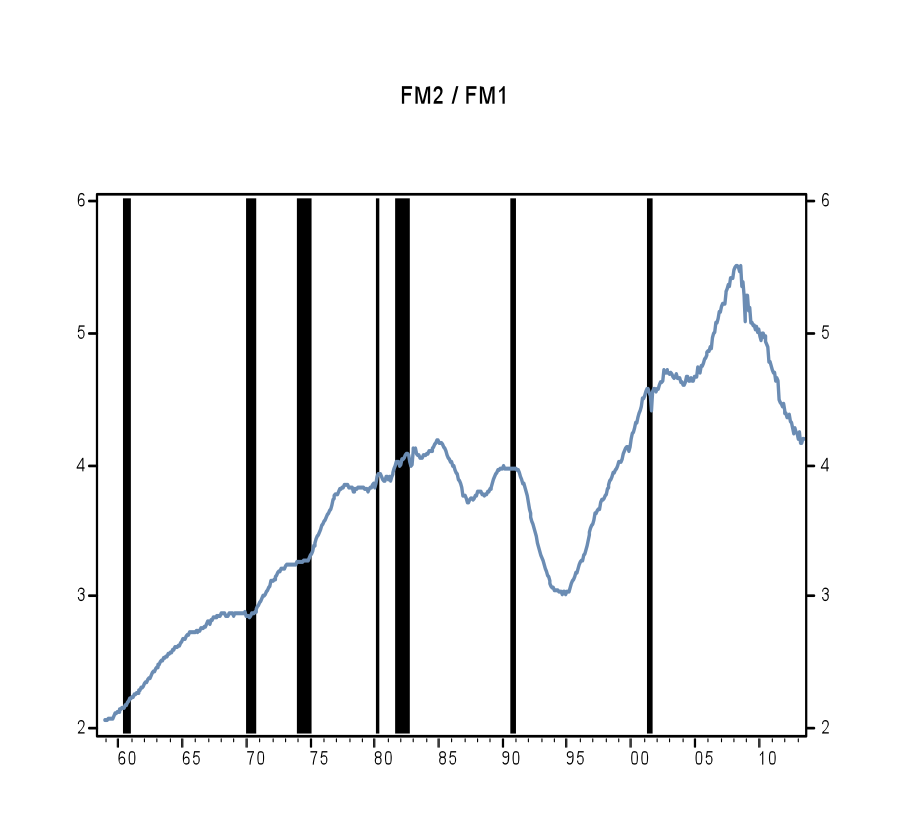
\includegraphics[width=1\linewidth]{figure/HistoricalFM.png}
  \caption*{}
  \label{fig:corp}
\end{subfigure}%
\centering
\begin{subfigure}{.30\textwidth}
  \centering
  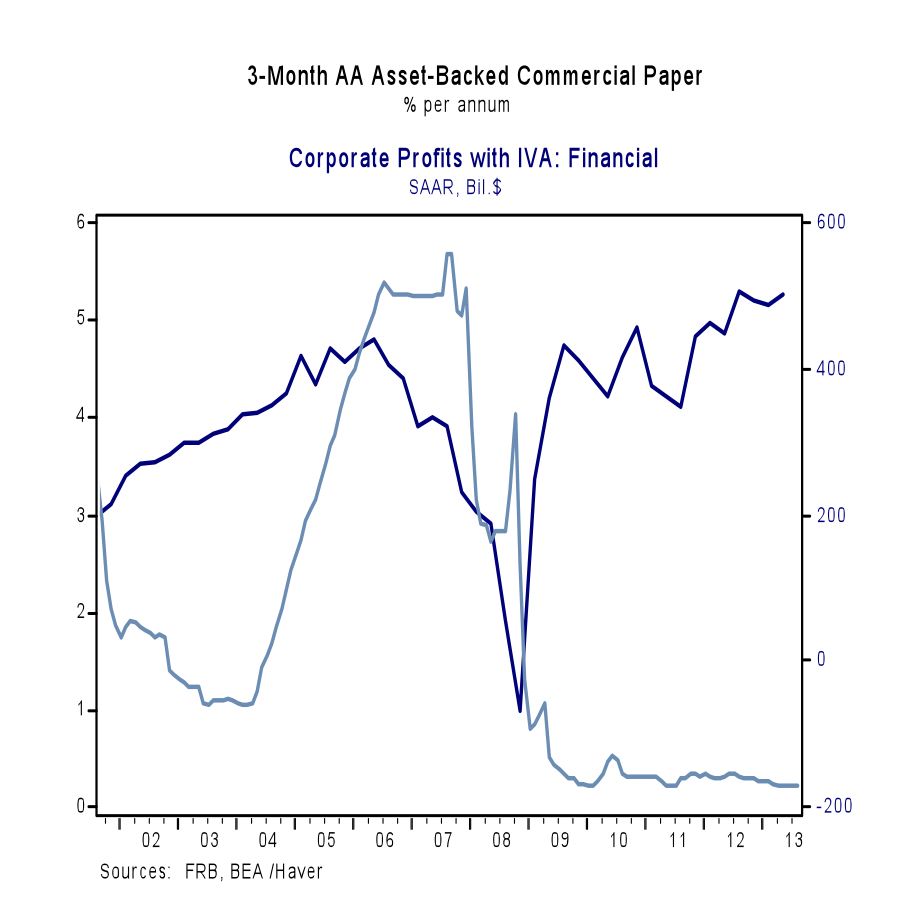
\includegraphics[width=1\linewidth]{figure/HugeRedFlag.png}
  \caption*{}
  \label{fig:corp}
\end{subfigure}%
\begin{subfigure}{.35\textwidth}
  \centering
  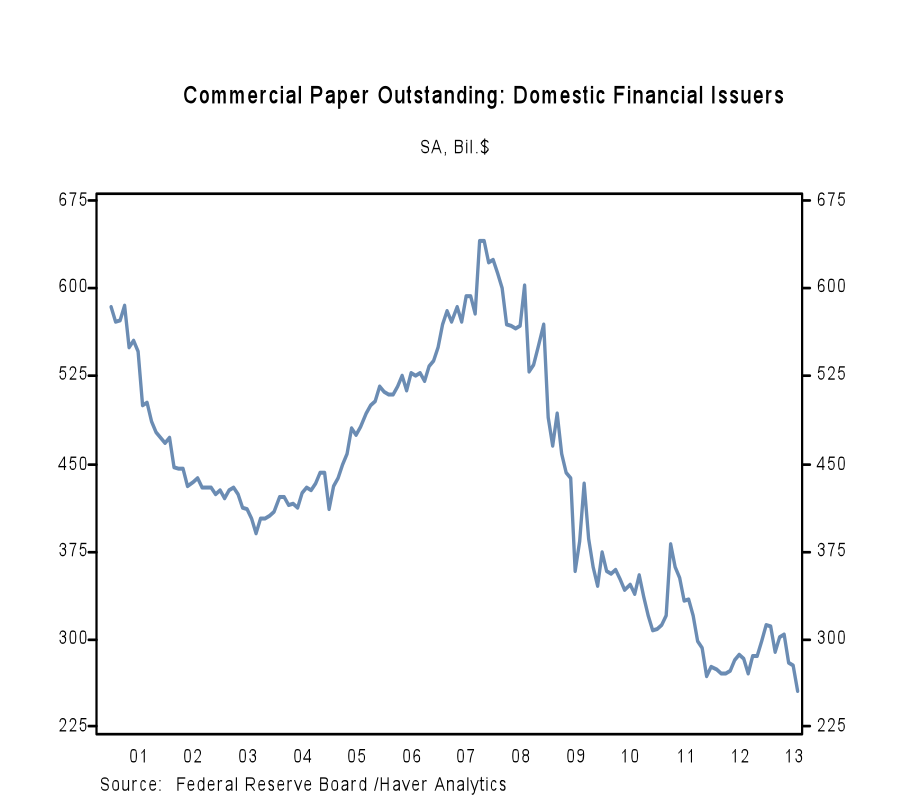
\includegraphics[width=1\linewidth]{figure/DomesticFinancial_CommPaper.png}
  \caption*{}
  \label{fig:muni}
\end{subfigure}\\[-1cm]
\caption{Impending TBTF}
\label{fig:TBTF}
\end{figure}

We postulate that in inherently leveraged fractional-banking systems the availability of credit and general setting of leverage can tell a lot about the recession to come and the stability in asset prices.  The United States economic researchers need to further develop models for this type of recession because the upward market leverage will leave the government responsible as not only the lender of last resort, but the lender of \textbf{only} resort.  


% Better understanding the general level of market discipline and stability:::: Re-title the paper, a Working understanding of market stability, through analysis of recent TBTF}

